\documentclass[a4paper]{article}
\usepackage[T1]{fontenc}
\usepackage{hyperref}
\usepackage[margin=1.1in]{geometry}
\usepackage{graphicx}
\usepackage{float}
\renewcommand{\figurename}{Zdjęcie}

\title{Określanie ilości osób na stoku narciarskim na podstawie nagrań wideo, w celu określenia obciążenia trasy\\
\small \url{https://github.com/szymon159/ski-slope-motion-detection}}
\date{}
\author{Michał Rogala, Szymon Stasiak, Przemysław Woźniakowski}

\begin{document}
  \maketitle

\section{Wstęp}
Projekt zrealizowany został w formie aplikacji desktopowej stworzonej z wykorzystaniem technologii \textit{.NET Framework}. Warstwa graficzna zaimplementowana z użyciem \textit{WPF}.\\
Przedstawiona aplikacja wczytuje pliki do analizy i przetworzenia oraz zapewnia podstawowe możliwości regulacji niektórych parametrów wywołań w celu lepszego dostosowania otrzymanego wyniku do potrzeb użytkownika.

\subsection{Cel}
Celem projektu było stworzenie aplikacji umożliwiającej narciarzom oraz osobom administrującym stokami narciarskimi analizę zapełnienia stoku, wraz z wyznaczaniem wyjątkowo eksploatowanych obszarów za pomocą nagrania.\\
Dzięki przetworzeniu nagrań za pomocą naszej aplikacji, użytkownik może w łatwy sposób pozyskać informacje dotyczące natężenia ruchu na stoku w zależności od czasu i miejsca. Dzięki temu stworzona aplikacja może stanowić pomoc w wyborze odpowiedniego czasu i miejsca wejścia na stok dla osób planujących wybranie się na niego.\\
Projekt miał również cel badawczy: w jego ramach chcieliśmy sprawdzić czy dość prosta i posiadająca ograniczenia metoda wykrywania ruchu bazująca na metodzie \textit{background subtractingu} (różnicy między klatką a tłem) może zostać wykorzystana do praktycznych celów przy odpowiednim zawężeniu wymagań i postawieniu sprecyzowanych przypadków użycia.

\subsection{Założenia}
W związku z panującą na świecie epidemią, dostęp do transmisji ze stoków jest niestety ograniczony, dlatego też w większości testów posłużyliśmy się archiwalnymi nagraniami z serwisu YouTube. Jako podstawowy materiał do testów zostało wybrane nagranie ze stoku Snoqualmie w USA dostępne w serwisie YouTube pod adresem (\url{https://youtube.com/watch?v=GNV9a4Ilsq8}).\\ 
Dominująca część analizy oparła się na ujęciach zaczynających się około 42. minuty tego nagrania (przykładowe klatki poniżej), założyliśmy więc:
\begin{itemize}
\item statyczną kamerę
\item mniej więcej stałą wielkość (procentową względem całości kadru) narciarza
\item dobre warunki atmosferyczne (dobra widoczność, jasność, kontrast)
\item brak dodatkowych elementów ruchomych (wyciągów itp.)
\item małe obciążenie stoku (poniżej 40 osób w dowolnym momencie)
\end{itemize}
Żadne z wymienionych założeń nie musi oznaczać ograniczenia (w szczególności program powinien działać sprawnie dla większej liczby narciarzy), jednak pozwalają określić minimalne wymagania, dla których projekt można uznać za zakończony powodzeniem.\\
W pierwszej części realizacji projektu skupiliśmy się na kadrach widocznych w minutach 44:06 - 46:54 (zdjęcie 1), później jako dodatkowe materiały przeanalizowaliśmy zachowanie dla innych ujęć (przykładowe zdjęcia 2 i 3).
\begin{figure}[H]
  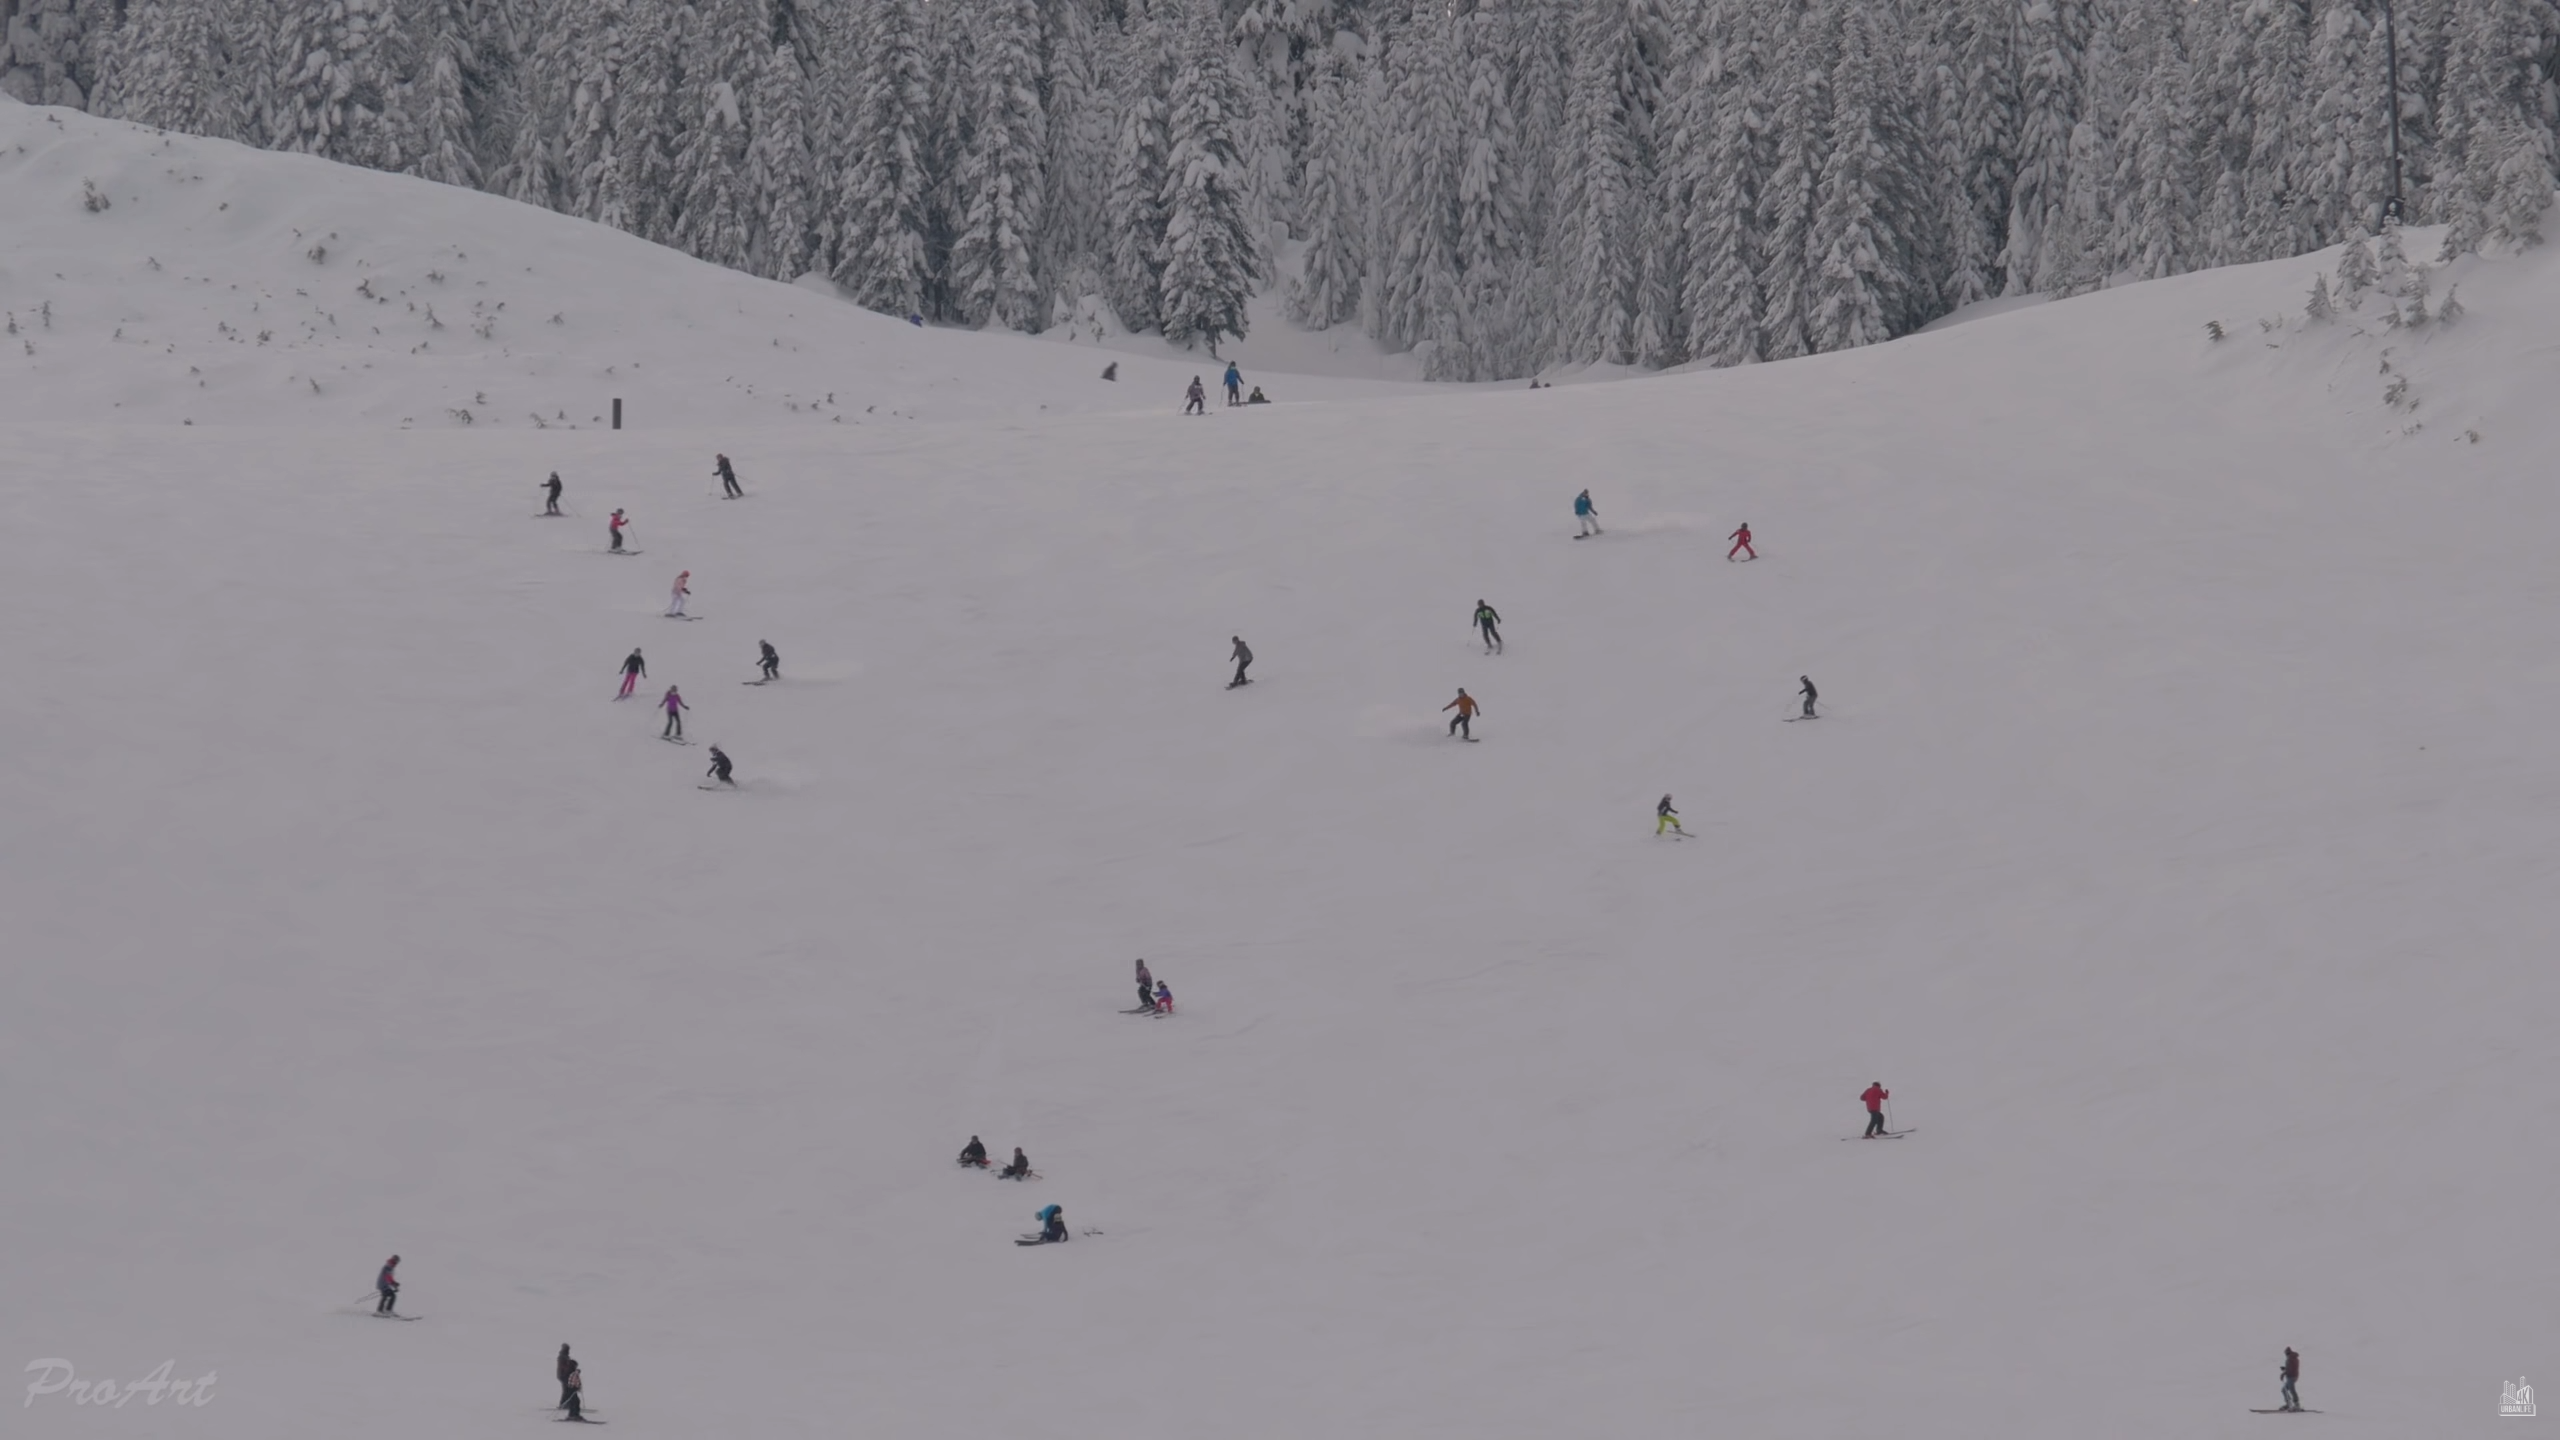
\includegraphics[width=\linewidth]{resources/img1.png}
  \caption{Podstawowe ujęcie}
\end{figure}
\begin{figure}[H]
  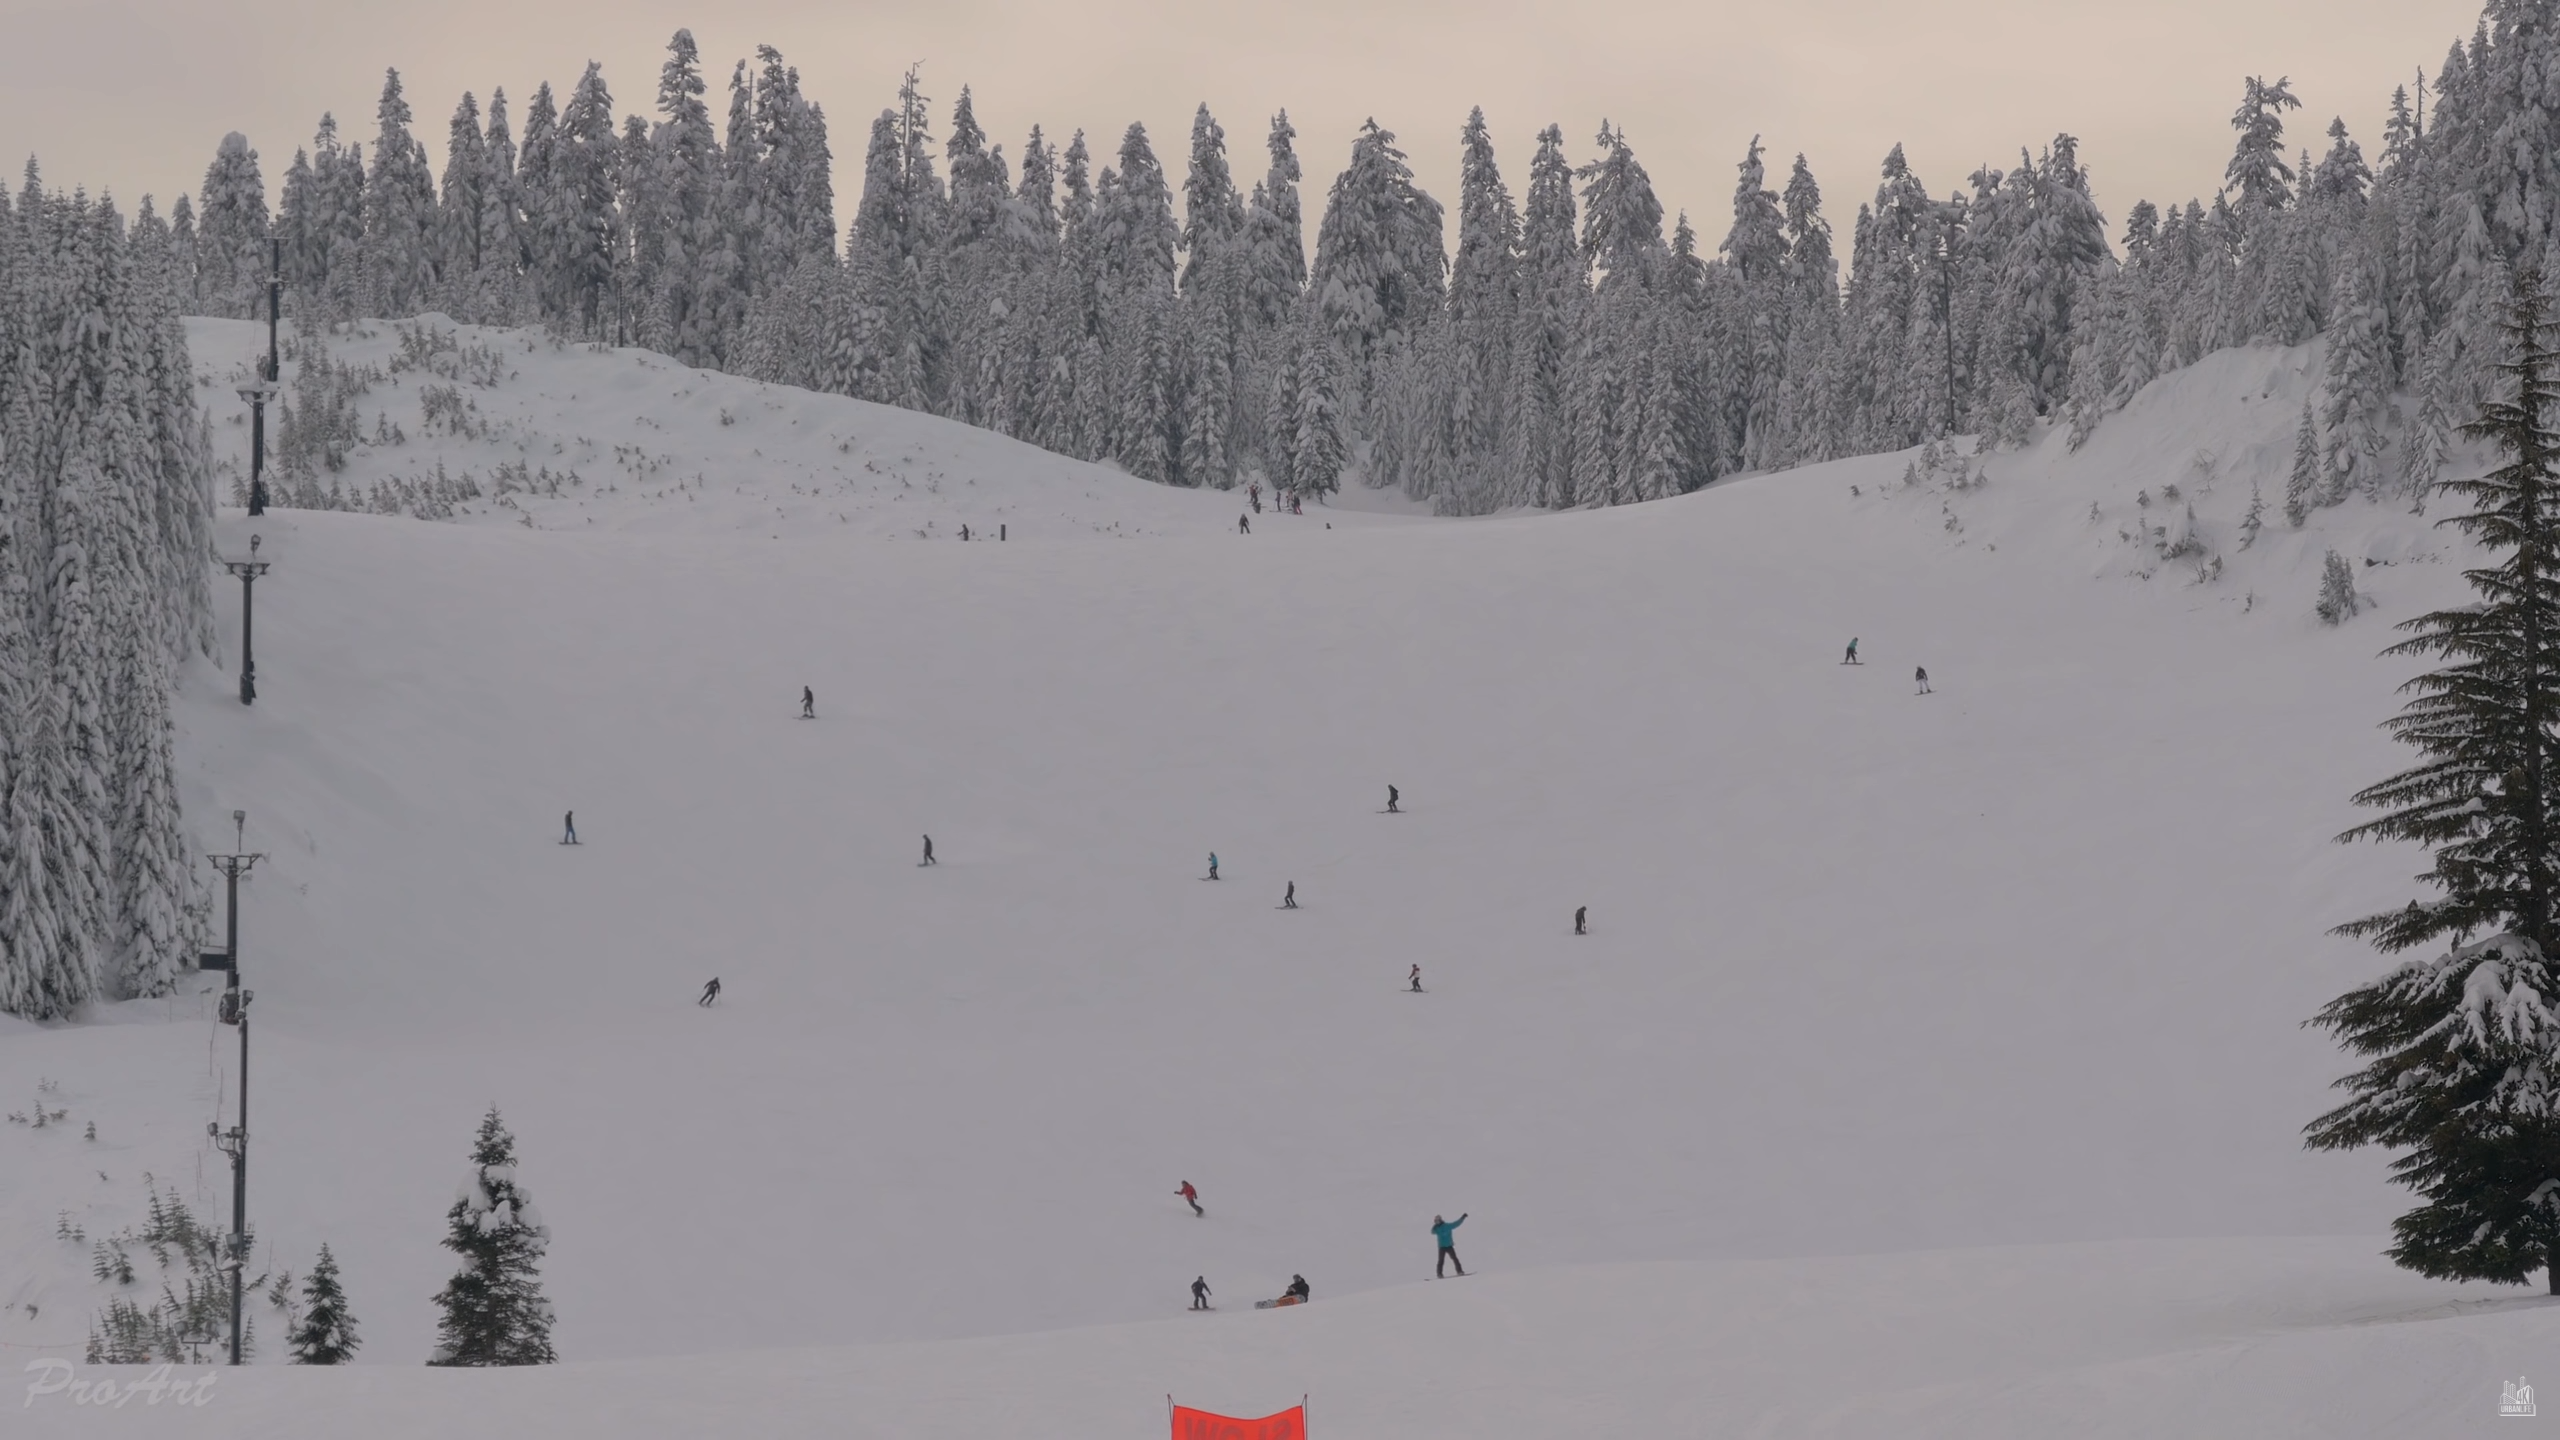
\includegraphics[width=\linewidth]{resources/img2.png}
  \caption{Ujęcie z dalszej perspektywy}
\end{figure}
\begin{figure}[H]
  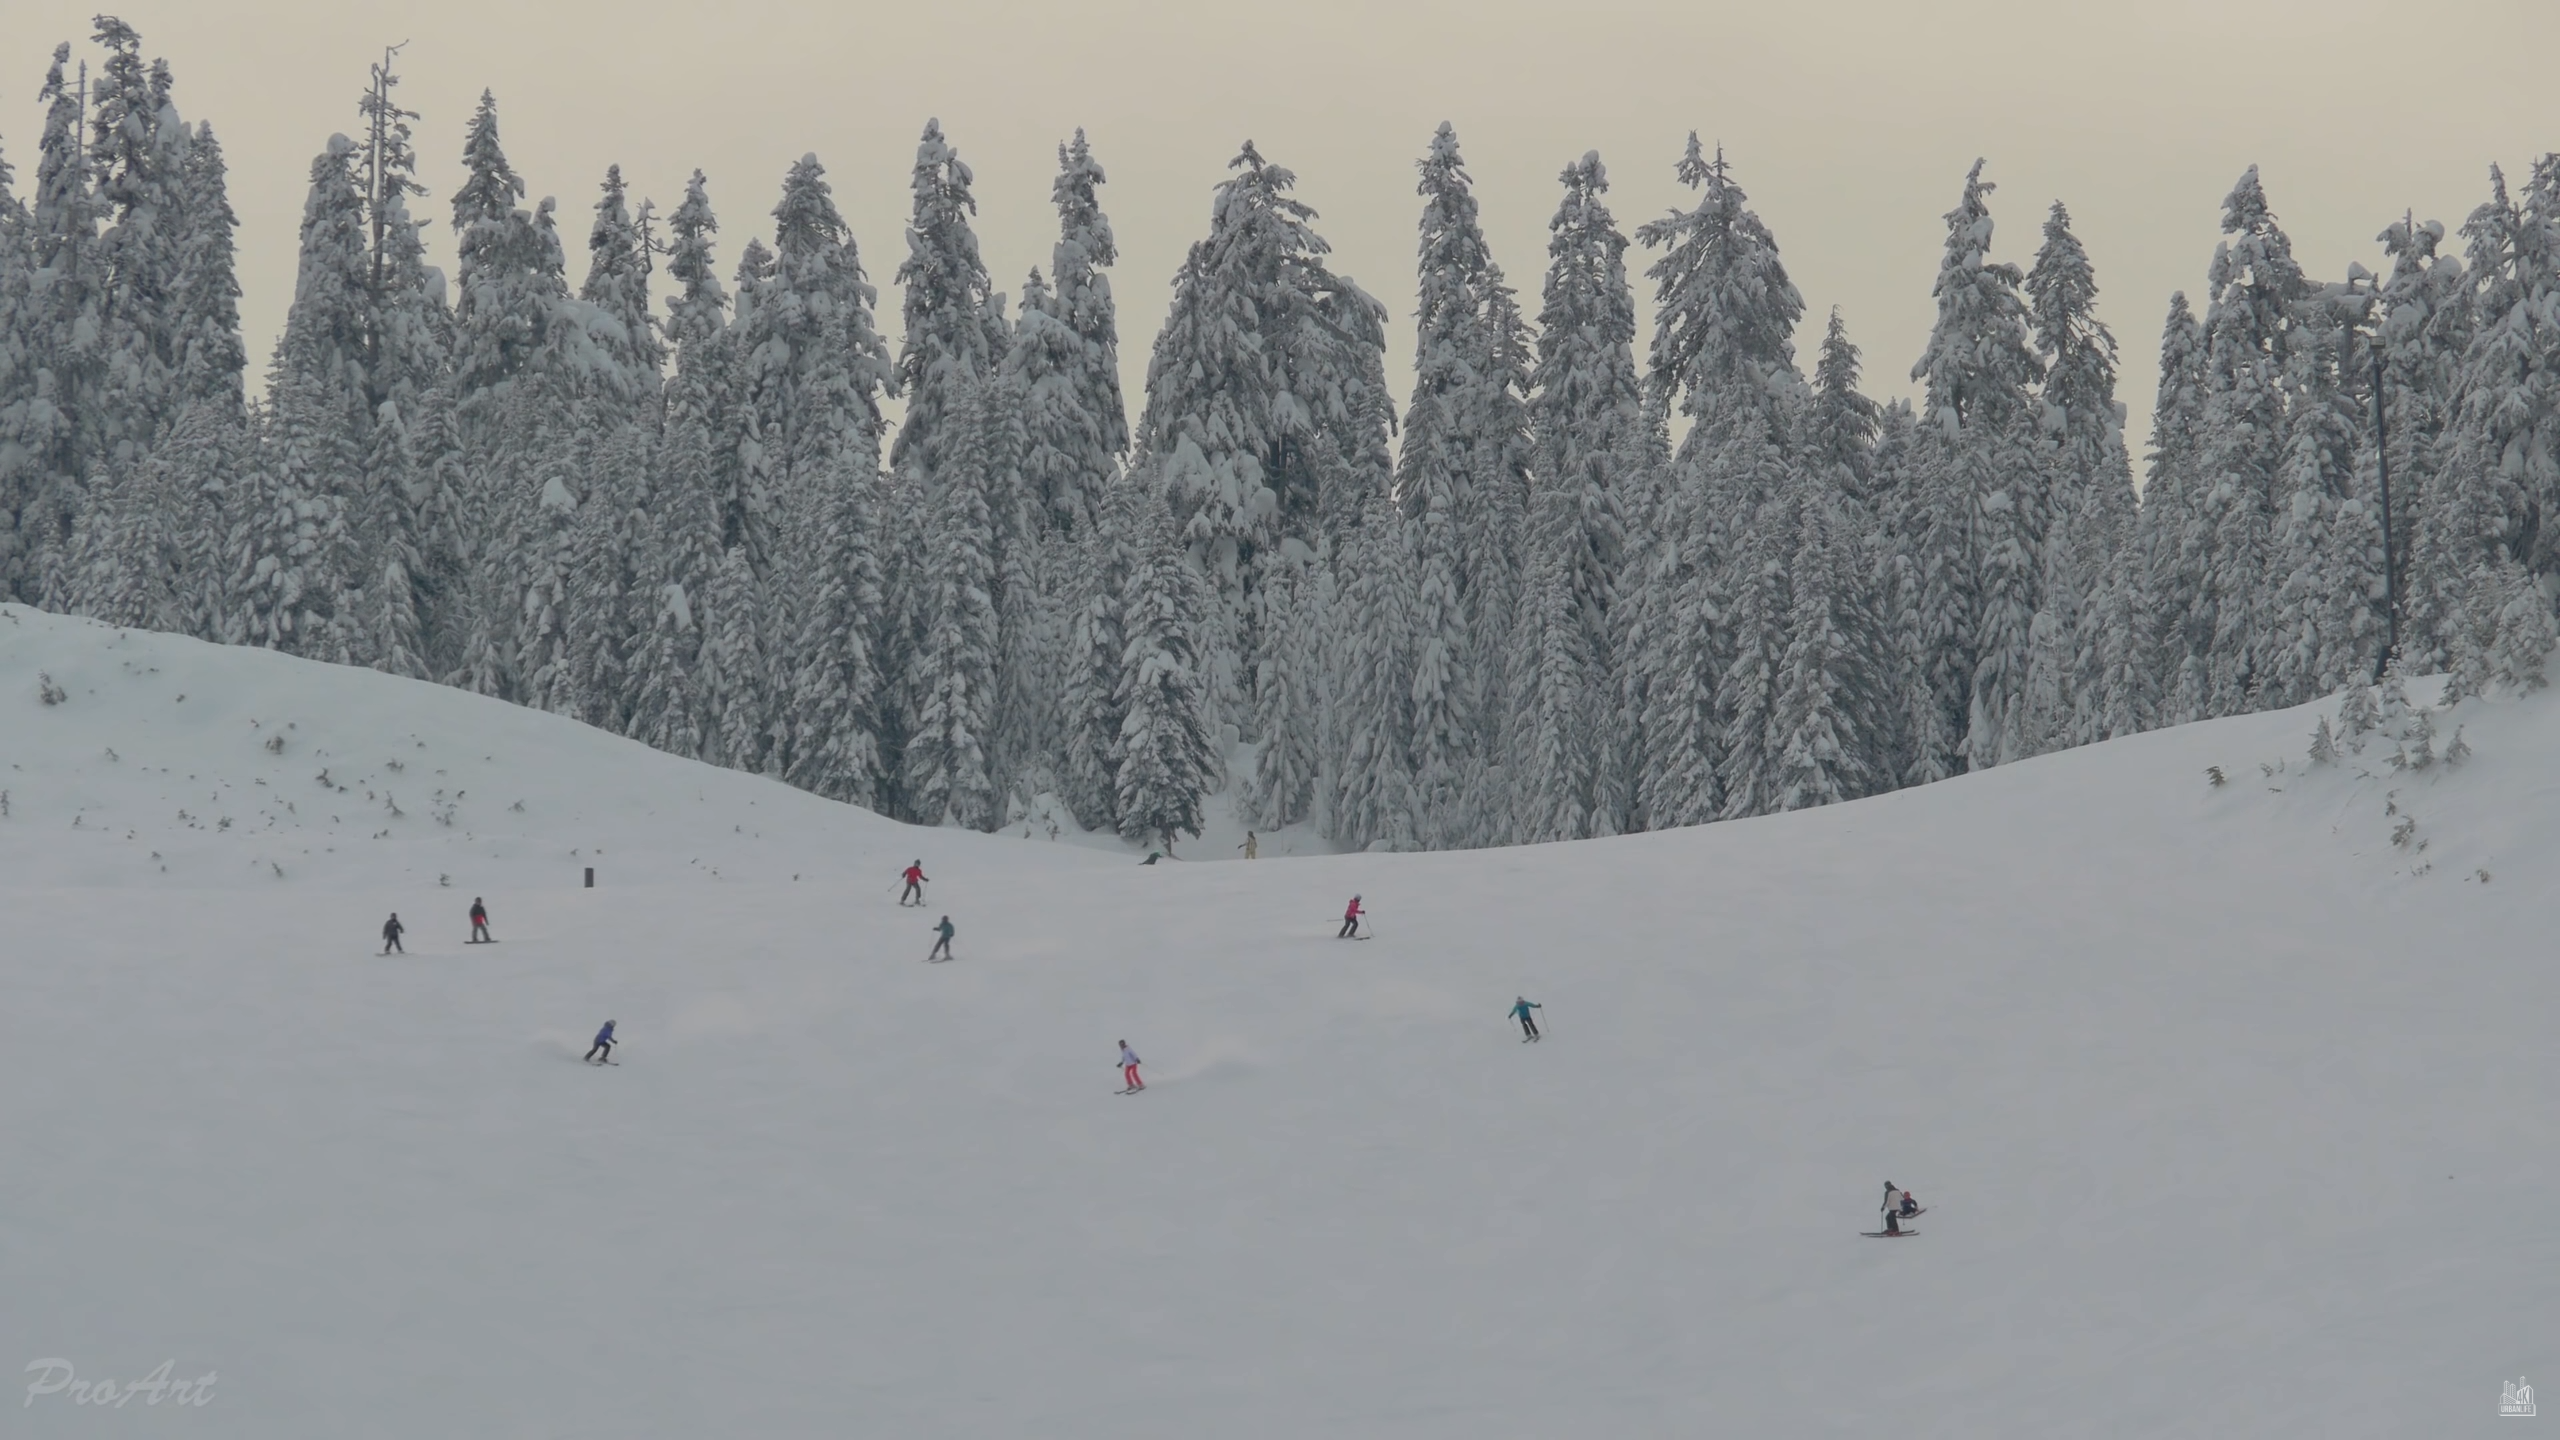
\includegraphics[width=\linewidth]{resources/img3.png}
  \caption{Większa powierzchnia tła}
\end{figure}

\section{Wykonane prace}
Prace wykonane w celu stworzenia aplikacji realizującej wspomniany cel można podzielić na kilka segmentów:
\begin{enumerate}
\item \textbf{Implementacja algorytmów przetwarzania wideo} – zgodnie z założeniami, zaimplementowane zostały dwie metody – metoda oparta na różnicach między kolejnymi klatkami oraz metoda naiwna oparta na wykrywaniu ciemnych plam na kolejnych klatkach nagrania. Więcej o zaimplementowanych metodach w sekcji \textit{\ref{sec:Methods} Zaimplementowane metody}
\item \textbf{Eksport danych} – w celu zobrazowania efektów działania algorytmów, w programie dodane zostało okno podglądu umożliwiające analizę nagrania na bieżąco, jak również zaimplementowane zostały różne metody eksportu, pozwalające użytkownikowi wybrać interesujący go efekt dla całego nagrania, bądź też jego części. Tak też dostępne opcje eksportu to:
\begin{itemize}
\item Obecna klatka z podglądu wideo wraz z zaznaczonymi narciarzami
\item Wideo z zaznaczonymi narciarzami  z możliwością wyboru zakresu klatek
\item Statystyki dotyczące średniej liczby użytkowników na stoku w określonym przedziale czasu (możliwość wyboru zakresu klatek oraz przedziału – sekunda, minuta, godzina)
\item Heatmapa przedstawiająca na tle stoku miejsca o największym zagęszczeniu ruchu w określonym przedziale klatek
\end{itemize}
\begin{figure}[H]
  \centering
  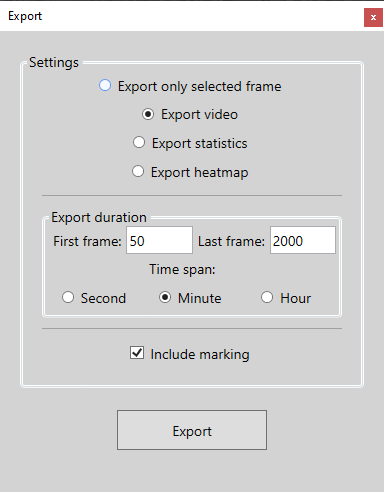
\includegraphics[width=0.4\linewidth]{resources/img4.png}
  \caption{Okno eksportu}
\end{figure}
\item \textbf{Budowa aplikacji} – dużym wyzwaniem było stworzenie aplikacji oferującej wspomniane funkcjonalności w optymalnym czasie, była to również najbardziej czasochłonna część projektu, jednak efekty pozwalają na względnie komfortowe korzystanie z metod nawet niezaawansowanym użytkownikom
\end{enumerate}
\begin{figure}[H]
  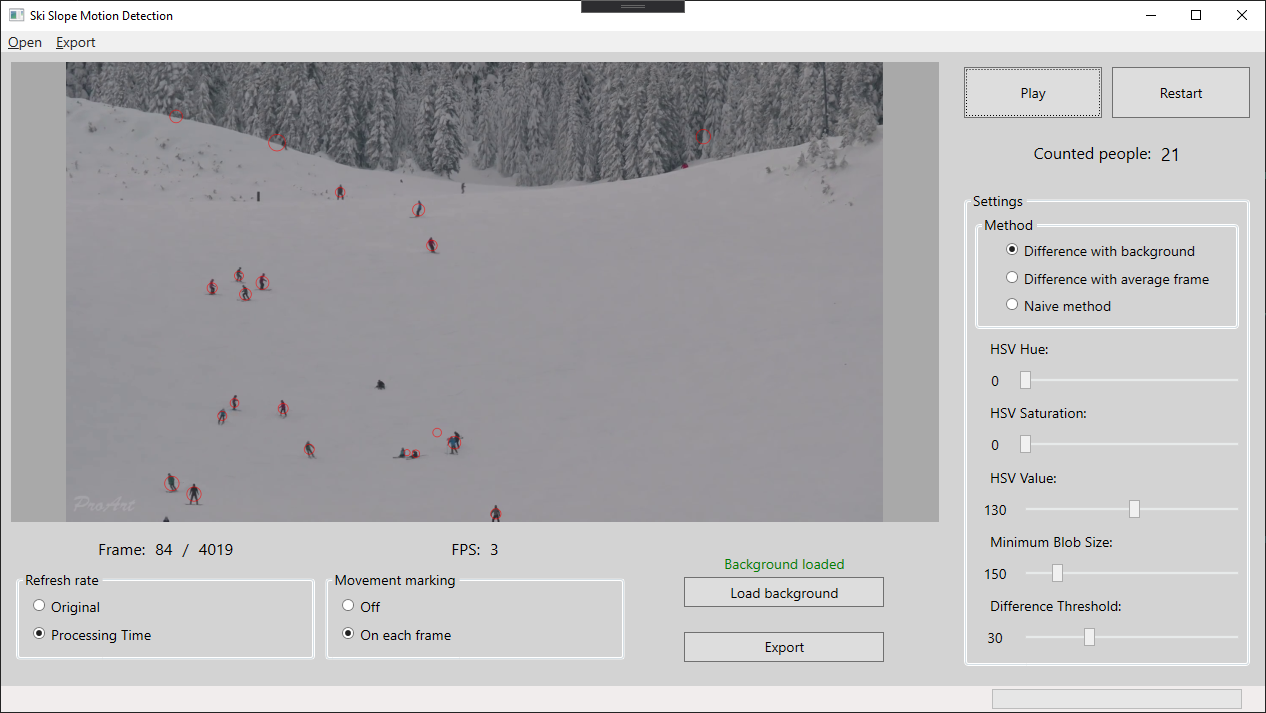
\includegraphics[width=\linewidth]{resources/img5.png}
  \caption{Główne okno aplikacji}
\end{figure}
Wykonane prace można również podzielić według osób odpowiedzialnych za wspomniane segmenty. Podział ten prezentuje się następująco: 
\begin{itemize}
\item Michał - opracowanie naiwnej metody oraz jej przetestowanie, pomoc przy tworzeniu interfejsu graficznego, przygotowanie kontrolek odpowiedzialnych za parametryzację. Implementacja komponentu odpowiedzialnego za liczenie średniej z klatek filmu podczas jego odtwarzania. 
\item Szymon – opracowanie interfejsu graficznego aplikacji, architektura, wczytywanie i eksport plików, ekstrakcja klatek. Implementacja własnego odtwarzacza wideo umożliwiającego operacje na osobnych klatkach wideo
\item Przemysław - wstępna implementacja metody background subtractingu ze średnią, wybór i rozpoznanie technologii \textit{EmguCV}, mechanizm wyciągania średniej z n klatek, tworzenie heatmapy.
\end{itemize}

\section{Metodyka}
Aplikacja została wykonana w języku \textit{C\#} w technologii \textit{WPF}, z wykorzystaniem bibliotek \textit{EmguCV}, \textit{Accord.Video} i \textit{OxyPlot}. Kod był tworzony w oparciu o paradygmaty programowania obiektowego z zachowaniem dobrych praktyk tworzenia aplikacji z interfejsem graficznym. Współpraca nad projektem przebiegała w ramach repozytorium na \textit{GitHubie}. 

\subsection{Zaimplementowane metody}
\label{sec:Methods}
\begin{enumerate}
\item \textbf{Detekcja i śledzenie ruchu używając obrazu tła i różnic między kolejnymi klatkami materiału wideo} (\textit{Motion Detection and Tracking using Background Subtraction and Consecutive Frames Difference Method})
	\begin{enumerate}
	\item Obraz tła uzyskany jako średnia z wielu klatek nagrania
	\item Obraz tła (pusty stok) wgrany z pliku
	\end{enumerate}
\item \textbf{Metoda naiwna} (\textit{Blob detection}) – wykrywanie ciemnych plan na kolejnych klatkach
	\begin{enumerate}
	\item Zróżnicowanie wyników w zależności od parametrów – zakresy wielkości "plam" uznawanych za narciarza, progi kolorów
	\end{enumerate}
\end{enumerate}	

\subsubsection{Metoda background subtractingu ze średnią klatką}
Metoda ta do porównywania wykorzystuje średnią z określonej liczby klatek pobieranych z filmu. Każdy piksel średniego obrazka jest otrzymywany przez zsumowanie składowych RGB z wszystkich odpowiadających mu pikseli z klatek, podzieleniu sumy przez ilość klatek i obcięcie do części całkowitych. Liczenie średniej odbywa się równolegle. Następnie średnia porównywana jest z daną klatką. Jeżeli różnica pomiędzy wartościami składowymi piksela na średniej klatce i na rozpatrywanej jest większa niż zadana tolerancja (threshold), to piksel jest zaznaczany na biało, w przeciwnym razie na czarno. Następnie na wynikowym obrazie uruchamiany jest algorytm detekcji tzw. blobów (białych obszarów) z dobranymi parametrami (rozmiar, okrągłość).
Schemat działania prezentuje się więc następująco:
\begin{enumerate}
\item Obliczenie średniej
\item Pobranie klatki do porównania
\item Wyznaczenie różnicy między klatkami
\item Detekcja blobów
\end{enumerate}

\subsubsection{Metoda background subtractingu z obrazem tła z pliku}
Metoda z tłem ma bardzo podobny schemat działania jak metoda ze średnią, jednak zamiast średniej, wykorzystywane jest w niej tło które dodajemy w aplikacji za pomocą przycisku.

\subsubsection{Metoda naiwna}
Metoda naiwna pozwala na względne oszacowanie liczby narciarzy na stoku, jednak jest mniej dokładna niż metody wykorzystujące średnia z tła filmu. Wymaga ona również dobierania parametrów na bieżąco w celu uzyskania rezultatów najbardziej zbliżonych do rzeczywistych wartości. Wydajność metody jest podobna do pozostałych metod. Działanie metody naiwnej:
\begin{enumerate}
\item Pobranie klatki do analizy.
\item Konwersja klatki do przestrzeni barw HSV.
\item Wybranie obszarów klatki, których składowe barwy są poniżej zadanego poziomu.
\item Policzenie uzyskanych w ten sposób obszarów. Pod uwagę brane są jedynie obszary większe od określonego przez parametr promienia.
\end{enumerate}

\section{Eksperymenty}
W trakcie implementowania rozwiązania, przeprowadziliśmy kilka eksperymentów mających na celu przybliżenie nas do osiągnięcia oczekiwanego rezultatu. Niestety najważniejsze z nich zakończyły się porażką.\\
W początkach implementacji metody naiwnej podjęta została próba bez wykorzystania konwersji do przestrzeni barw HSV.  Efektem była zdecydowanie mniejsza dokładność metody oraz losowe punkty z otoczenia miały większy udział w liczbie wykrytych narciarzy. Z tego powodu w finalnej wersji owa konwersja została wprowadzona. Szczęśliwie nie miała ona znacznego wpływu na szybkość działania algorytmu.\\
Innym istotnym podejściem była próba użycia wektorów ruchu wykorzystywanych w kompresji MPEG. Niestety, jak się okazało, nie istnieje żadna metoda dostępna dla platformy \textit{.NET} umożliwiająca odzyskanie tych wektorów. Żaden z dostępnych wrapperów na \textit{FFMPEG} nie udostępnia tej funkcji, mimo iż wspomniany \textit{FFMPEG} daje taką możliwość. Z tego powodu zrezygnowaliśmy z implementacji tej metody. \\
Kolejnym eksperymentem, wykraczającym poza przyjęte założenia, było przetestowanie metody dla nagrania stoku z kamery umieszczonej na kasku zjeżdżającego narciarza. Dało ono zaskakująco dobre przybliżenie liczby osób znajdujących się w polu widzenia. Niestety momentami duża część zliczeń pochodziła z tła, jednak jest to zrozumiały efekt zważywszy na to, że obraz nie jest statyczny. Nagranie to wymagało również zwiększenia thresholdu (przedstawione na poniższych zdjęciach 6, 7).
\begin{figure}[H]
  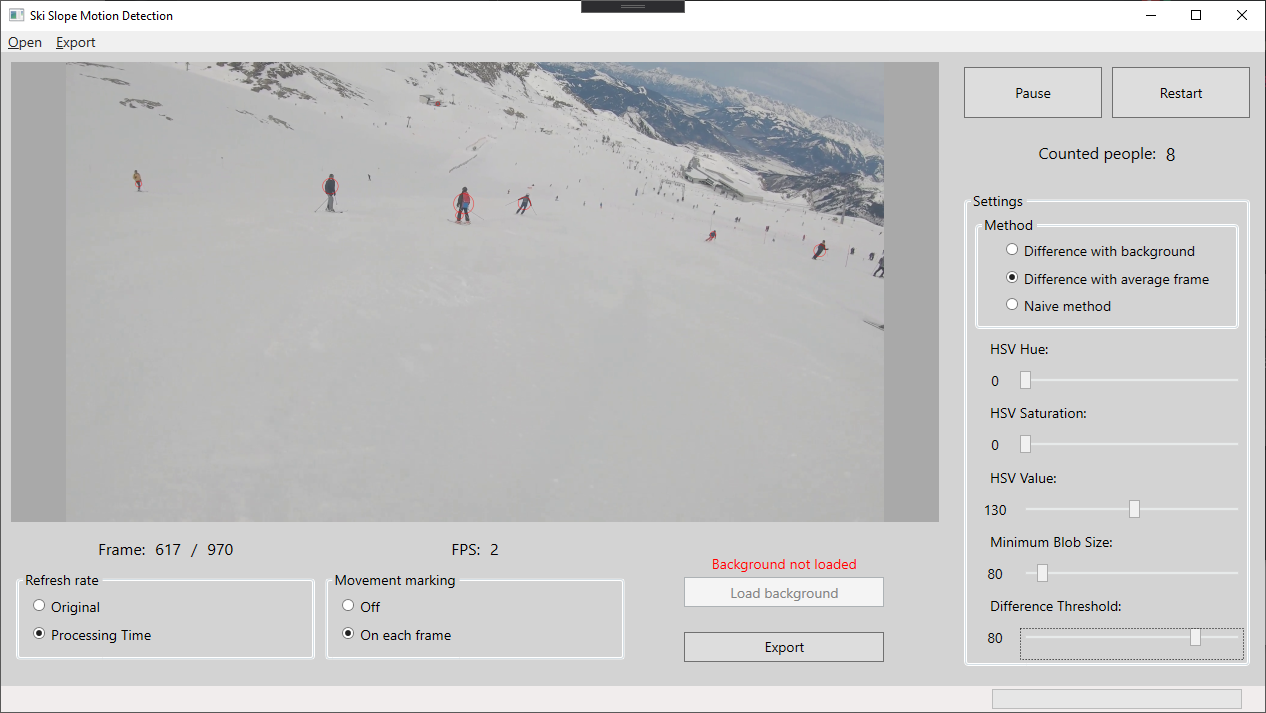
\includegraphics[width=\linewidth]{resources/img6.png}
  \caption{Analiza dla nagrania z kasku zjeżdżającego narciarza}
\end{figure}
\begin{figure}[H]
  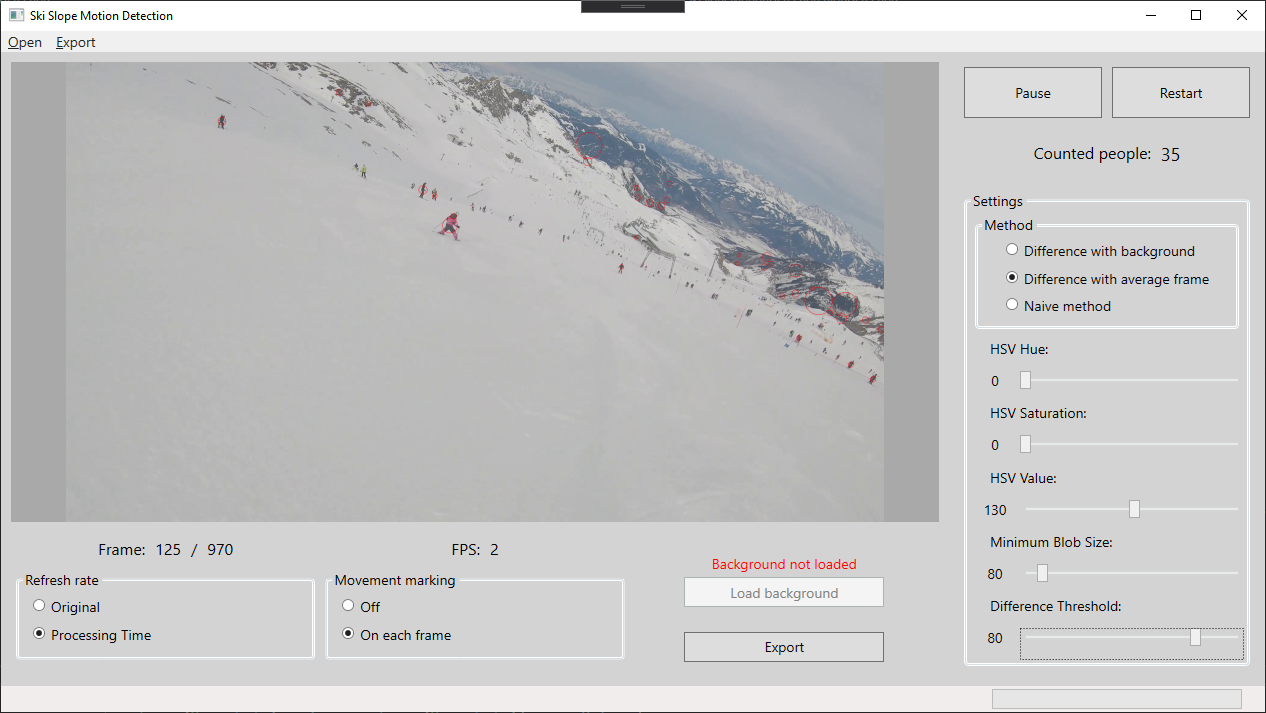
\includegraphics[width=\linewidth]{resources/img7.png}
  \caption{Analiza dla nagrania z kasku zjeżdżającego narciarza wraz z błędnie zaznaczonymi elementami tła}
\end{figure}

\section{Wyniki}
Jako zbiór testowy nagrań posłużyły nam wspomniane wcześniej 3 ujęcia tego samego stoku (zdjęcia 1, 2 oraz 3). Dla każdego z nagrań przeprowadziliśmy testy opierające się na eksporcie danych dla detekcji różnymi metodami a następnie na porównaniu otrzymanych rezultatów z wartością realną. Niestety, z powodu niemożności uzyskania sensownego obrazu tła dla ujęcia drugiego i trzeciego, pominięte zostały analizy metody z obrazem tła dla tych ujęć. Ponadto, w celu zoptymalizowania pracy, wartość realna liczona była wyłącznie co 10-15 sekund, stąd znaczne różnice w kształtach poniższych wykresów.\\
\begin{figure}[H]
  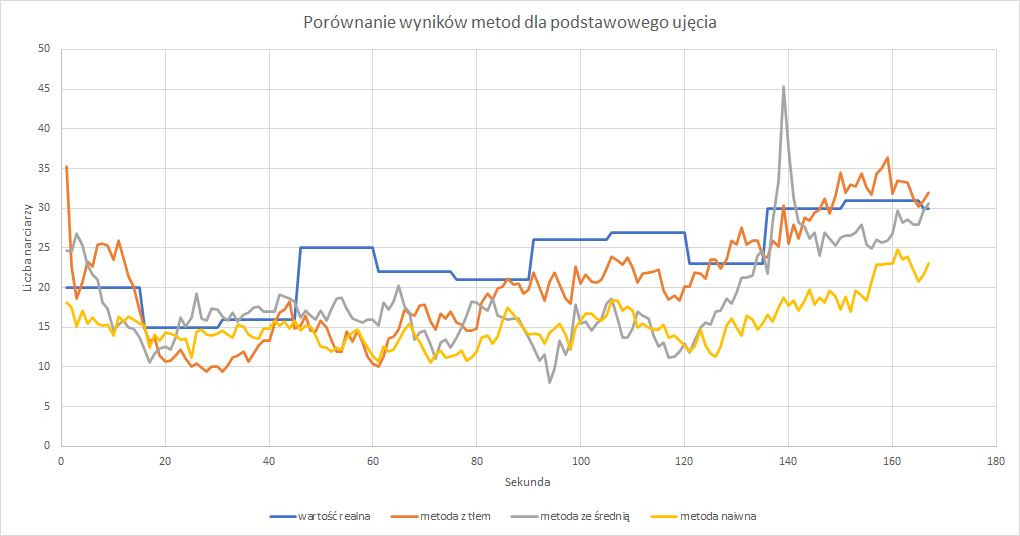
\includegraphics[width=\linewidth]{resources/img8.png}
  \caption{Analiza dla ujęcia podstawowego}
\end{figure}
\begin{figure}[H]
  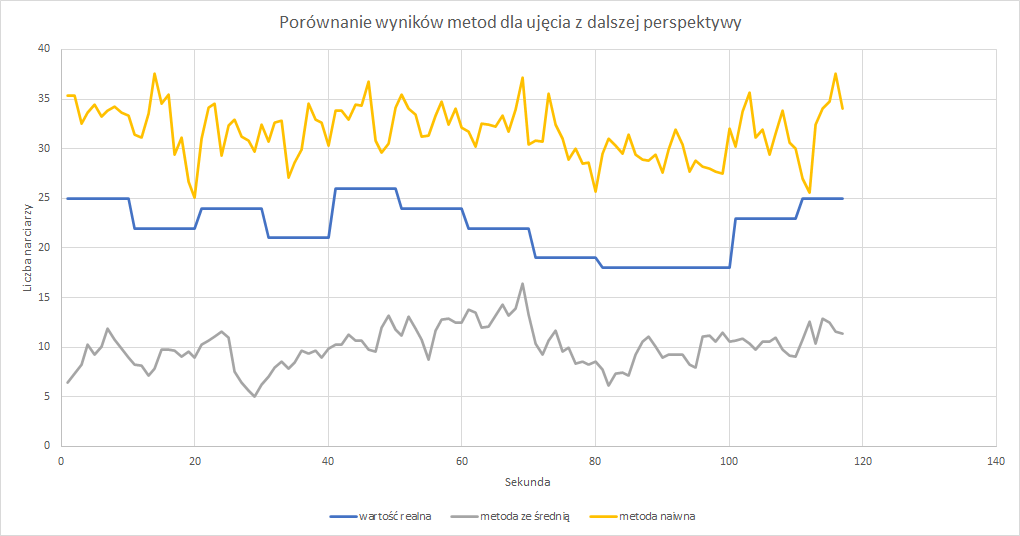
\includegraphics[width=\linewidth]{resources/img9.png}
  \caption{Analiza dla ujęcia z dalszej perspektywy}
\end{figure}
\begin{figure}[H]
  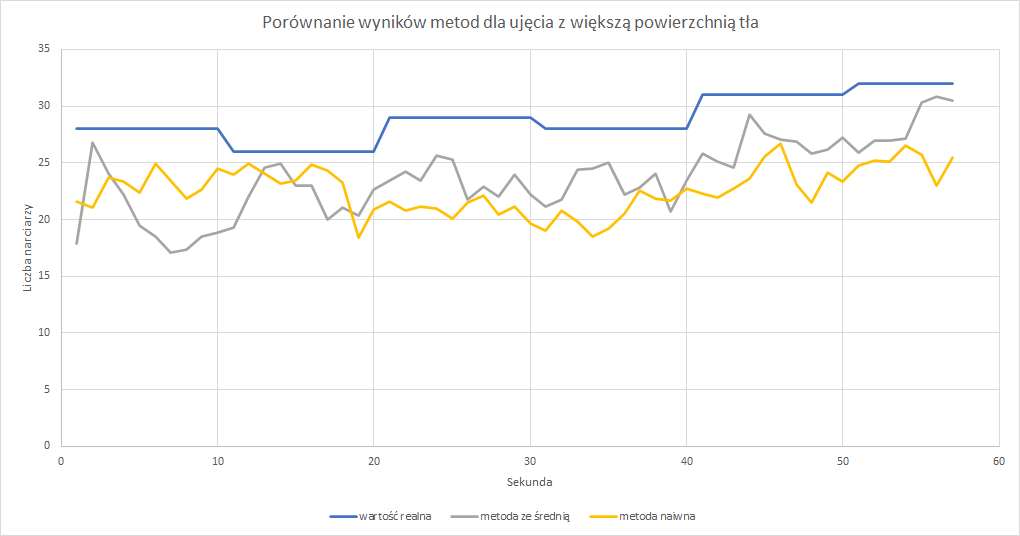
\includegraphics[width=\linewidth]{resources/img10.png}
  \caption{Analiza dla ujęcia z większą powierzchnią tła}
\end{figure}

Ponadto, dla każdego nagrania wygenerowaliśmy również heatmapy, w tym przypadku jednak korzystając tylko z jednej metody - metody \textit{background subtractingu} z wykorzystaniem klatki średniej.
%\begin{figure}[H]
%  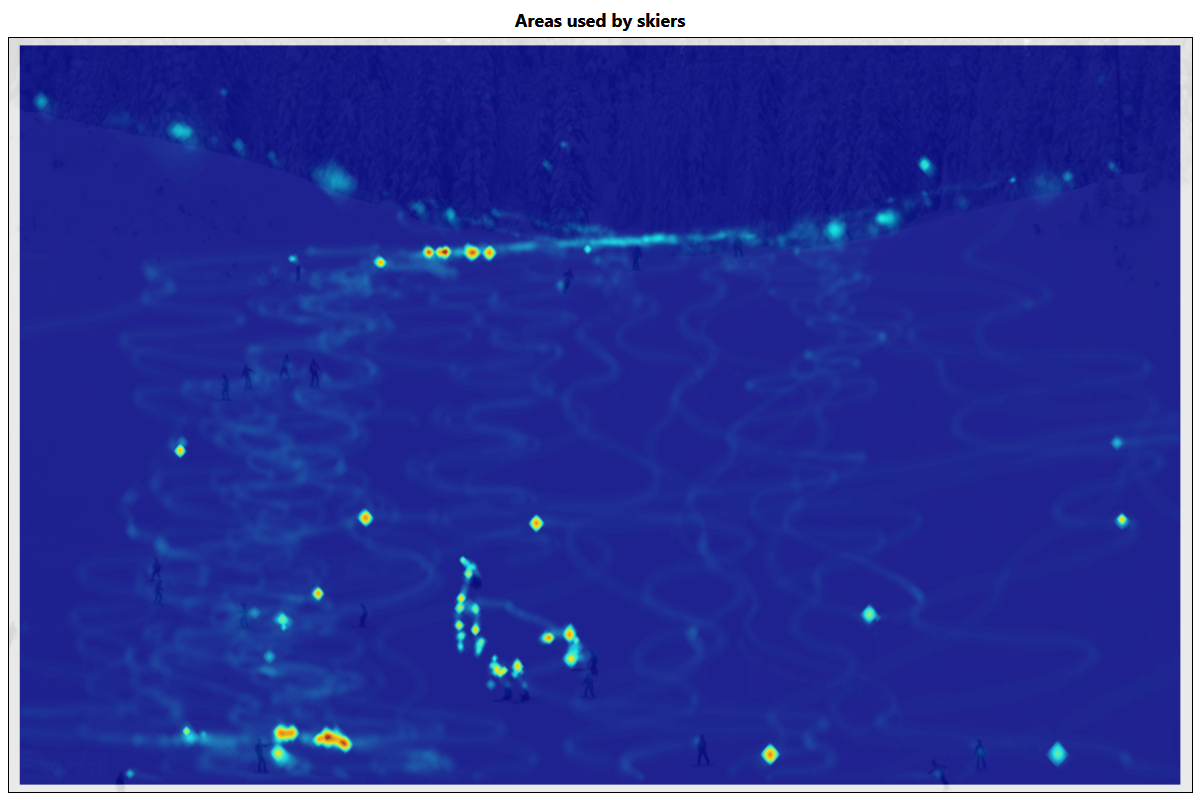
\includegraphics[width=\linewidth]{resources/img11.png}
%  \caption{Heatmapa dla ujęcia podstawowego}
%\end{figure}
%\begin{figure}[H]
%  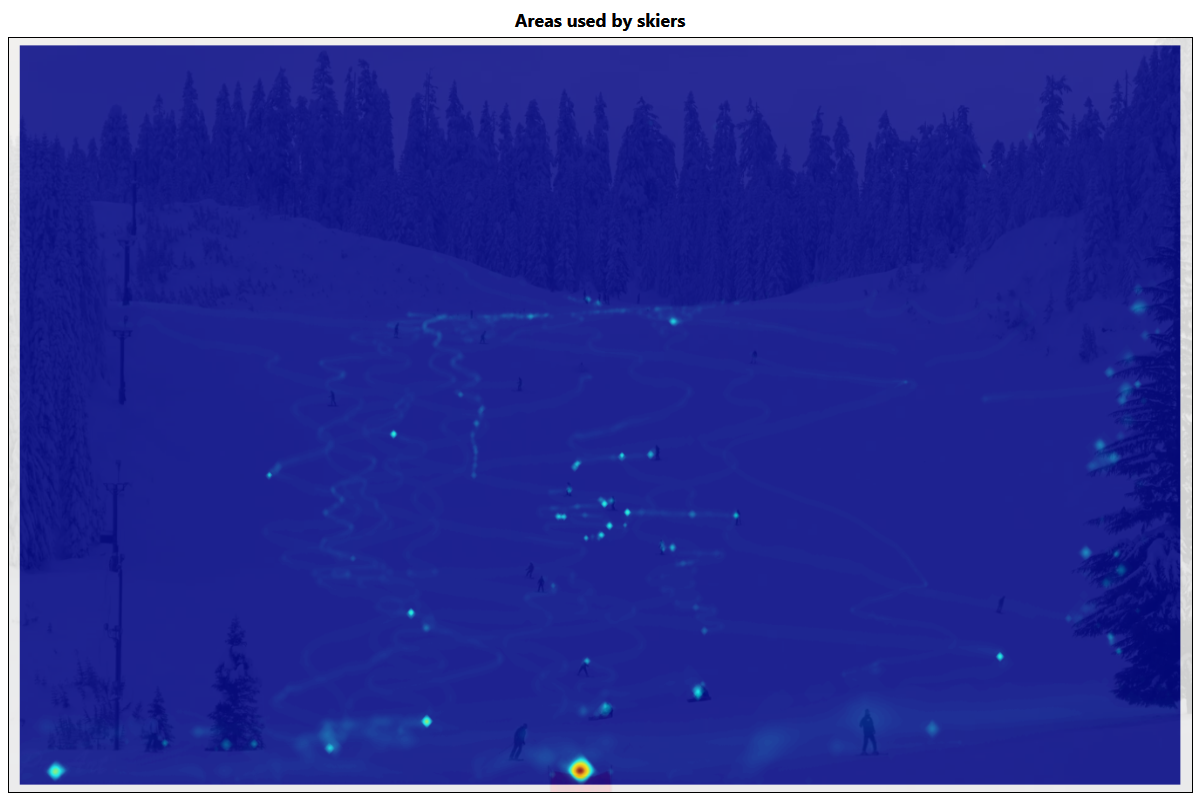
\includegraphics[width=\linewidth]{resources/img12.png}
%  \caption{Heatmapa dla ujęcia z dalszej perspektywy}
%\end{figure}
%\begin{figure}[H]
%  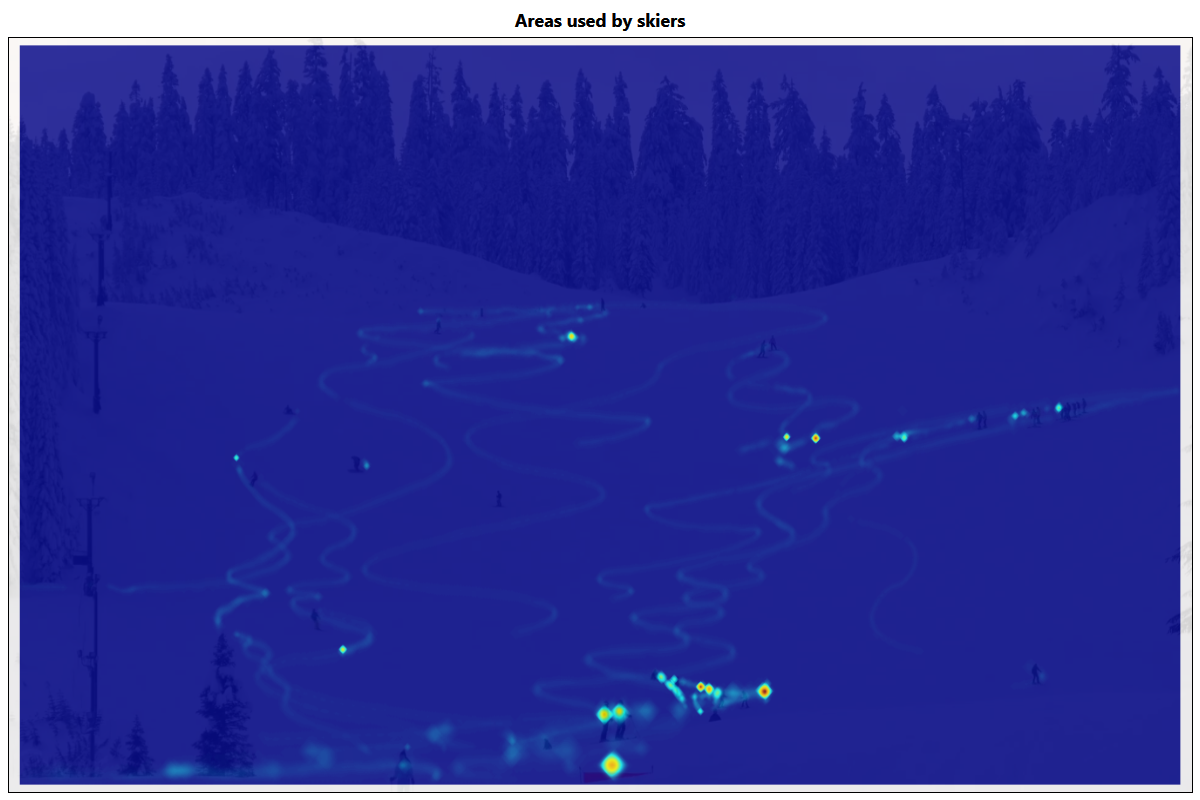
\includegraphics[width=\linewidth]{resources/img13.png}
%  \caption{Heatmapa dla ujęcia z większą powierzchnią tła}
%\end{figure}

Jak widać po heatmapach, większość narciarzy porusza się po bardzo zbliżonych trasach. Dodatkowo wyraźne zaznaczenie owych tras pozwala, w uzupełnieniu o własne doświadczenie i obserwację wideo, uznać iż wyniki prezentowane przez heatmapę odzwierciedlają rzeczywistą sytuację na stoku.

\section{Ocena efektów}
Pomimo iż aplikacja została ukończona, uważamy, że postawione przez nas cele nie zostały osiągnięte w stopniu satysfakcjonującym.\\
Aplikacja z powodu konieczności obliczania średniej ze znacznej ilości klatek  przy głównej metodzie nie działa tak płynnie jak z początku zakładaliśmy (osiąga poniżej 10 klatek na sekundę), jednak na tyle płynnie, że jest to akceptowalna w odbiorze prędkość. Na płynność odtwarzania istotny wpływ ma fakt, że potrzebna jest ekstrakcja kolejnych klatek filmu oraz ich przetworzenie.\\
Metoda \textit{background subtractingu}, tak jak oczekiwaliśmy, okazała się  być najlepszym wyborem spośród zaimplementowanych przez nas podejść, jednak ona również posiada widoczne mankamenty przy stosowaniu jej w naszym programie. Dzieje się tak głównie ze względu na dodatkowe obiekty takie jak kamienie lub drzewa, które mogą znajdować się na stoku poza narciarzami i śniegiem, a mogą zostać omyłkowo wzięte za narciarza. Co prawda aplikacja pozwala na manipulowanie opcjami wykrywania, jednak ich możliwości również są ograniczone, a dodatkowo konieczność ingerencji użytkownika, demaskuje wady tej metody.\\
Niestety płynność działania aplikacji przekreśla możliwość używania jej na większą skalę niż uczelniany projekt. Tempo przetwarzania około 10 klatek na sekundę było co prawda przewidywane, jednak dla filmu o 24 klatkach na sekundę, daje to czas przetwarzania 2.5 razy większy od czasu właściwego filmu. Stąd też analiza jednego dnia na stoku (7h), zajęłaby naszemu algorytmowi całą dobę. Jest to czas nieakceptowalny dla przeciętnego użytkownika.

\section{Wnioski}
Zastosowana w projekcie analiza poklatkowa wideo okazała się metodą niezwykle zasobochłonną. Pamięć RAM wykorzystywana przez program niemal nieustannie osiągała maksimum udostępnione przez system. Narzut wynikający z zastosowanej technologii również wpływał negatywnie na osiągi programu. Jasno narzuca się zatem wniosek, iż wybierając wspomnianą technologię, w zamian za nie najwyższy poziom skomplikowania implementacyjnego, ponieśliśmy koszty w kwestii osiągów programu. Interesującą szansą usprawnienia aplikacji jest wykorzystanie obliczeń wspomaganych przez procesory graficzne dla operacji na mapach bitowych.\\
Ponadto zdaliśmy sobie sprawę, że przyjęta przez nas metodyka nie była w stu procentach poprawna. Z racji, że postawiliśmy sobie za cel zbadanie możliwości naszych metod, momentami zamiast dobierać odpowiednie metody do funkcjonalności, modyfikowaliśmy funkcjonalność by pasowała do naszych metod. Jest to ważna lekcja na przyszłość i następnym razem przy rozwiązywaniu podobnego problemu, przyjęlibyśmy inne podejście.

\end{document}

